\documentclass[twoside]{book}

% Packages required by doxygen
\usepackage{fixltx2e}
\usepackage{calc}
\usepackage{doxygen}
\usepackage{graphicx}
\usepackage[utf8]{inputenc}
\usepackage{makeidx}
\usepackage{multicol}
\usepackage{multirow}
\PassOptionsToPackage{warn}{textcomp}
\usepackage{textcomp}
\usepackage[nointegrals]{wasysym}
\usepackage[table]{xcolor}

% Font selection
\usepackage[T1]{fontenc}
\usepackage{mathptmx}
\usepackage[scaled=.90]{helvet}
\usepackage{courier}
\usepackage{amssymb}
\usepackage{sectsty}
\renewcommand{\familydefault}{\sfdefault}
\allsectionsfont{%
  \fontseries{bc}\selectfont%
  \color{darkgray}%
}
\renewcommand{\DoxyLabelFont}{%
  \fontseries{bc}\selectfont%
  \color{darkgray}%
}
\newcommand{\+}{\discretionary{\mbox{\scriptsize$\hookleftarrow$}}{}{}}

% Page & text layout
\usepackage{geometry}
\geometry{%
  a4paper,%
  top=2.5cm,%
  bottom=2.5cm,%
  left=2.5cm,%
  right=2.5cm%
}
\tolerance=750
\hfuzz=15pt
\hbadness=750
\setlength{\emergencystretch}{15pt}
\setlength{\parindent}{0cm}
\setlength{\parskip}{0.2cm}
\makeatletter
\renewcommand{\paragraph}{%
  \@startsection{paragraph}{4}{0ex}{-1.0ex}{1.0ex}{%
    \normalfont\normalsize\bfseries\SS@parafont%
  }%
}
\renewcommand{\subparagraph}{%
  \@startsection{subparagraph}{5}{0ex}{-1.0ex}{1.0ex}{%
    \normalfont\normalsize\bfseries\SS@subparafont%
  }%
}
\makeatother

% Headers & footers
\usepackage{fancyhdr}
\pagestyle{fancyplain}
\fancyhead[LE]{\fancyplain{}{\bfseries\thepage}}
\fancyhead[CE]{\fancyplain{}{}}
\fancyhead[RE]{\fancyplain{}{\bfseries\leftmark}}
\fancyhead[LO]{\fancyplain{}{\bfseries\rightmark}}
\fancyhead[CO]{\fancyplain{}{}}
\fancyhead[RO]{\fancyplain{}{\bfseries\thepage}}
\fancyfoot[LE]{\fancyplain{}{}}
\fancyfoot[CE]{\fancyplain{}{}}
\fancyfoot[RE]{\fancyplain{}{\bfseries\scriptsize Generated on Sat Nov 22 2014 13\+:49\+:43 for Teacher by Doxygen }}
\fancyfoot[LO]{\fancyplain{}{\bfseries\scriptsize Generated on Sat Nov 22 2014 13\+:49\+:43 for Teacher by Doxygen }}
\fancyfoot[CO]{\fancyplain{}{}}
\fancyfoot[RO]{\fancyplain{}{}}
\renewcommand{\footrulewidth}{0.4pt}
\renewcommand{\chaptermark}[1]{%
  \markboth{#1}{}%
}
\renewcommand{\sectionmark}[1]{%
  \markright{\thesection\ #1}%
}

% Indices & bibliography
\usepackage{natbib}
\usepackage[titles]{tocloft}
\setcounter{tocdepth}{3}
\setcounter{secnumdepth}{5}
\makeindex

% Hyperlinks (required, but should be loaded last)
\usepackage{ifpdf}
\ifpdf
  \usepackage[pdftex,pagebackref=true]{hyperref}
\else
  \usepackage[ps2pdf,pagebackref=true]{hyperref}
\fi
\hypersetup{%
  colorlinks=true,%
  linkcolor=blue,%
  citecolor=blue,%
  unicode%
}

% Custom commands
\newcommand{\clearemptydoublepage}{%
  \newpage{\pagestyle{empty}\cleardoublepage}%
}


%===== C O N T E N T S =====

\begin{document}

% Titlepage & ToC
\hypersetup{pageanchor=false,
             bookmarks=true,
             bookmarksnumbered=true,
             pdfencoding=unicode
            }
\pagenumbering{roman}
\begin{titlepage}
\vspace*{7cm}
\begin{center}%
{\Large Teacher }\\
\vspace*{1cm}
{\large Generated by Doxygen 1.8.8}\\
\vspace*{0.5cm}
{\small Sat Nov 22 2014 13:49:43}\\
\end{center}
\end{titlepage}
\clearemptydoublepage
\tableofcontents
\clearemptydoublepage
\pagenumbering{arabic}
\hypersetup{pageanchor=true}

%--- Begin generated contents ---
\chapter{Teacher\+Basic}
\label{md___users_nishantjain__desktop__developing_programming__teacehr_basics__r_e_a_d_m_e}
\hypertarget{md___users_nishantjain__desktop__developing_programming__teacehr_basics__r_e_a_d_m_e}{}
A teacher program that teaches users about basics objects in C programming. 
\chapter{File Index}
\section{File List}
Here is a list of all files with brief descriptions\+:\begin{DoxyCompactList}
<<<<<<< HEAD
\item\contentsline{section}{Developing\+Programming/\+Teacher\+Basics/\hyperlink{_teacher_basics_8c}{Teacher\+Basics.\+c} }{\pageref{_teacher_basics_8c}}{}
=======
\item\contentsline{section}{/\+Users/nishantjain/\+Desktop/\+Developing\+Programming/\+Teacehr\+Basics/\hyperlink{_teacher_basics_8c}{Teacher\+Basics.\+c} }{\pageref{_teacher_basics_8c}}{}
>>>>>>> master
\end{DoxyCompactList}

\chapter{File Documentation}
\hypertarget{_r_e_a_d_m_e_8md}{\section{Developing\+Programming/\+Developing\+Computer\+Programming/\+R\+E\+A\+D\+M\+E.md File Reference}
\label{_r_e_a_d_m_e_8md}\index{Developing\+Programming/\+Developing\+Computer\+Programming/\+R\+E\+A\+D\+M\+E.\+md@{Developing\+Programming/\+Developing\+Computer\+Programming/\+R\+E\+A\+D\+M\+E.\+md}}
}

<<<<<<< HEAD
\hypertarget{_teacher_basics_8c}{\section{Developing\+Programming/\+Teacher\+Basics/\+Teacher\+Basics.c File Reference}
\label{_teacher_basics_8c}\index{Developing\+Programming/\+Teacher\+Basics/\+Teacher\+Basics.\+c@{Developing\+Programming/\+Teacher\+Basics/\+Teacher\+Basics.\+c}}
}
{\ttfamily \#include $<$stdio.\+h$>$}\\*
{\ttfamily \#include $<$string.\+h$>$}\\*
Include dependency graph for Teacher\+Basics.\+c\+:\nopagebreak
\begin{figure}[H]
\begin{center}
\leavevmode
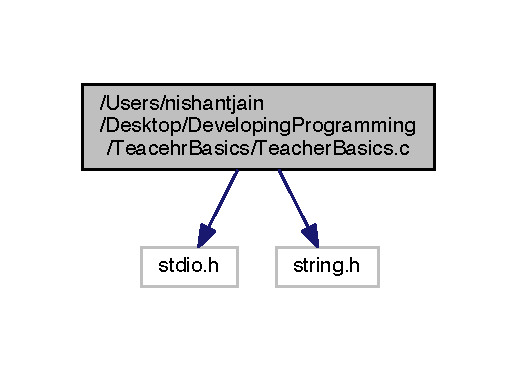
\includegraphics[width=242pt]{_teacher_basics_8c__incl}
=======
\hypertarget{_teacher_basics_8c}{\section{/\+Users/nishantjain/\+Desktop/\+Developing\+Programming/\+Teacehr\+Basics/\+Teacher\+Basics.c File Reference}
\label{_teacher_basics_8c}\index{/\+Users/nishantjain/\+Desktop/\+Developing\+Programming/\+Teacehr\+Basics/\+Teacher\+Basics.\+c@{/\+Users/nishantjain/\+Desktop/\+Developing\+Programming/\+Teacehr\+Basics/\+Teacher\+Basics.\+c}}
}
{\ttfamily \#include $<$stdio.\+h$>$}\\*
{\ttfamily \#include $<$string.\+h$>$}\\*
Include dependency graph for Teacher\+Basics.\+c\+:
\nopagebreak
\begin{figure}[H]
\begin{center}
\leavevmode
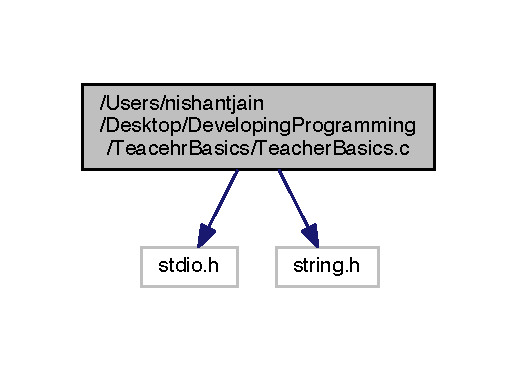
\includegraphics[width=248pt]{_teacher_basics_8c__incl}
>>>>>>> master
\end{center}
\end{figure}
\subsection*{Functions}
\begin{DoxyCompactItemize}
\item 
void \hyperlink{_teacher_basics_8c_ad0bea7ca09a6fd8663f0c0f7ac219c20}{Data\+Types} ()
\item 
void \hyperlink{_teacher_basics_8c_a6ef0cf8d139194a7cc30e0c64e09b14e}{Modifiers} ()
\item 
int \hyperlink{_teacher_basics_8c_ae66f6b31b5ad750f1fe042a706a4e3d4}{main} ()
\end{DoxyCompactItemize}
\subsection*{Variables}
\begin{DoxyCompactItemize}
\item 
const int \hyperlink{_teacher_basics_8c_af7dbda7167e22cb3417c16f78061ad80}{M\+A\+X} =2
\end{DoxyCompactItemize}


\subsection{Function Documentation}
\hypertarget{_teacher_basics_8c_ad0bea7ca09a6fd8663f0c0f7ac219c20}{\index{Teacher\+Basics.\+c@{Teacher\+Basics.\+c}!Data\+Types@{Data\+Types}}
\index{Data\+Types@{Data\+Types}!Teacher\+Basics.\+c@{Teacher\+Basics.\+c}}
\subsubsection[{Data\+Types}]{\setlength{\rightskip}{0pt plus 5cm}void Data\+Types (
\begin{DoxyParamCaption}
{}
\end{DoxyParamCaption}
)}}\label{_teacher_basics_8c_ad0bea7ca09a6fd8663f0c0f7ac219c20}


<<<<<<< HEAD
Definition at line 63 of file Teacher\+Basics.\+c.
=======
Definition at line 45 of file Teacher\+Basics.\+c.
>>>>>>> master



Referenced by main().


\begin{DoxyCode}
<<<<<<< HEAD
64 \{
65   \textcolor{comment}{//local variable, array}
66   \textcolor{keywordtype}{char} ch[10];                                                          
67   printf(\textcolor{stringliteral}{"\(\backslash\)nThere are four basic data types: char-character, "}
68   \textcolor{stringliteral}{"int-integer, float, and double. \(\backslash\)n"});
69   \textcolor{keywordtype}{int} i;
70   
71   \textcolor{keywordflow}{do}                                                                    
72   \{
73     printf(\textcolor{stringliteral}{"Which data type do you want to learn about? \(\backslash\)n"});
74     scanf(\textcolor{stringliteral}{" %s"}, ch);
75     i=0;
76     
77     \textcolor{comment}{/*}
78 \textcolor{comment}{    * Conditions for user's choice of subject. }
79 \textcolor{comment}{    * Following can be interpreted as a database of req. info. on subject}
80 \textcolor{comment}{    * Using <strcmp> to compare strings}
81 \textcolor{comment}{    */}
82     \textcolor{keywordflow}{if}(strcmp(ch,\textcolor{stringliteral}{"char"})==0) 
83     printf(\textcolor{stringliteral}{"char is a data type used to store a single"}
84     \textcolor{stringliteral}{" character such as a number, text or special characters."}
85     \textcolor{stringliteral}{"\(\backslash\)nStorage size:1 byte \(\backslash\)nValue Range:-128 to 127 or 0 to 255 \(\backslash\)n"}); 
86     \textcolor{keywordflow}{else} \textcolor{keywordflow}{if}(strcmp(ch,\textcolor{stringliteral}{"int"})==0) 
87     printf(\textcolor{stringliteral}{"int is a data type used to store numerical data. \(\backslash\)n"}
88     \textcolor{stringliteral}{" Storage size:2 bytes  \(\backslash\)nValue Range:-32,768 to 32,767  \(\backslash\)n"}); 
89     \textcolor{keywordflow}{else} \textcolor{keywordflow}{if}(strcmp(ch,\textcolor{stringliteral}{"float"})==0) 
90     printf(\textcolor{stringliteral}{"float is a data type used"}
91     \textcolor{stringliteral}{" to store decimal numbers up to 6 decimal places. \(\backslash\)n Storage"}
92     \textcolor{stringliteral}{" size:4 byte  \(\backslash\)nValue Range:1.2E-38 to 3.4E+38 \(\backslash\)n"}); 
93     \textcolor{keywordflow}{else} \textcolor{keywordflow}{if}(strcmp(ch,\textcolor{stringliteral}{"double"})==0) 
94     printf(\textcolor{stringliteral}{"double is a data type used"}
95     \textcolor{stringliteral}{" to store decimal numbers to up to 15 decimal places . \(\backslash\)n Storage size:8 byte"}
96     \textcolor{stringliteral}{"\(\backslash\)nValue Range:2.3E-308 to 1.7E+308 \(\backslash\)n"}); 
97     \textcolor{keywordflow}{else} 
98     \{ 
99       \textcolor{comment}{//Repeating the input if an error}
100       printf(\textcolor{stringliteral}{"Input either 'char', 'int', 'float' or 'double'. \(\backslash\)n"}); i=1;
101     \}               
102   \}\textcolor{keywordflow}{while}(i==1);
103   
104 \}
=======
46 \{
47   \textcolor{comment}{//local variable, array}
48   \textcolor{keywordtype}{char} ch[10];                                                          
49   printf(\textcolor{stringliteral}{"\(\backslash\)nThere are four basic data types: char-character, "}
50   \textcolor{stringliteral}{"int-integer, float, and double. \(\backslash\)n"});
51   \textcolor{keywordtype}{int} i;
52   
53   \textcolor{keywordflow}{do}                                                                    
54   \{
55     printf(\textcolor{stringliteral}{"Which data type do you want to learn about? \(\backslash\)n"});
56     scanf(\textcolor{stringliteral}{" %s"}, ch);
57     i=0;
58     
59     \textcolor{comment}{/*}
60 \textcolor{comment}{    * Conditions for user's choice of subject. }
61 \textcolor{comment}{    * Following can be interpreted as a database of req. info. on subject}
62 \textcolor{comment}{    * Using <strcmp> to compare strings}
63 \textcolor{comment}{    */}
64     \textcolor{keywordflow}{if}(strcmp(ch,\textcolor{stringliteral}{"char"})==0) 
65     printf(\textcolor{stringliteral}{"char is a data type used to store a single"}
66     \textcolor{stringliteral}{" character such as a number, text or special characters."}
67     \textcolor{stringliteral}{"\(\backslash\)nStorage size:1 byte \(\backslash\)nValue Range:-128 to 127 or 0 to 255 \(\backslash\)n"}); 
68     \textcolor{keywordflow}{else} \textcolor{keywordflow}{if}(strcmp(ch,\textcolor{stringliteral}{"int"})==0) 
69     printf(\textcolor{stringliteral}{"int is a data type used to store numerical data. \(\backslash\)n"}
70     \textcolor{stringliteral}{" Storage size:2 bytes  \(\backslash\)nValue Range:-32,768 to 32,767  \(\backslash\)n"}); 
71     \textcolor{keywordflow}{else} \textcolor{keywordflow}{if}(strcmp(ch,\textcolor{stringliteral}{"float"})==0) 
72     printf(\textcolor{stringliteral}{"float is a data type used"}
73     \textcolor{stringliteral}{" to store decimal numbers up to 6 decimal places. \(\backslash\)n Storage"}
74     \textcolor{stringliteral}{" size:4 byte  \(\backslash\)nValue Range:1.2E-38 to 3.4E+38 \(\backslash\)n"}); 
75     \textcolor{keywordflow}{else} \textcolor{keywordflow}{if}(strcmp(ch,\textcolor{stringliteral}{"double"})==0) 
76     printf(\textcolor{stringliteral}{"double is a data type used"}
77     \textcolor{stringliteral}{" to store decimal numbers to up to 15 decimal places . \(\backslash\)n Storage size:8 byte"}
78     \textcolor{stringliteral}{"\(\backslash\)nValue Range:2.3E-308 to 1.7E+308 \(\backslash\)n"}); 
79     \textcolor{keywordflow}{else} 
80     \{ 
81       \textcolor{comment}{//Repeating the input if an error}
82       printf(\textcolor{stringliteral}{"Input either 'char', 'int', 'float' or 'double'. \(\backslash\)n"}); i=1;
83     \}               
84   \}\textcolor{keywordflow}{while}(i==1);
85   
86 \}
>>>>>>> master
\end{DoxyCode}


Here is the caller graph for this function\+:\nopagebreak
\begin{figure}[H]
\begin{center}
\leavevmode
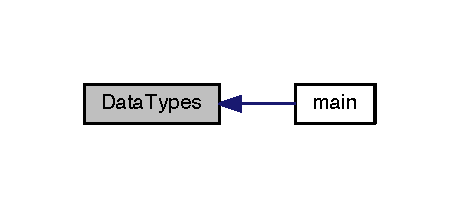
\includegraphics[width=220pt]{_teacher_basics_8c_ad0bea7ca09a6fd8663f0c0f7ac219c20_icgraph}
\end{center}
\end{figure}


\hypertarget{_teacher_basics_8c_ae66f6b31b5ad750f1fe042a706a4e3d4}{\index{Teacher\+Basics.\+c@{Teacher\+Basics.\+c}!main@{main}}
\index{main@{main}!Teacher\+Basics.\+c@{Teacher\+Basics.\+c}}
\subsubsection[{main}]{\setlength{\rightskip}{0pt plus 5cm}int main (
\begin{DoxyParamCaption}
{}
\end{DoxyParamCaption}
)}}\label{_teacher_basics_8c_ae66f6b31b5ad750f1fe042a706a4e3d4}
<<<<<<< HEAD
2 do-\/while loops 9 if-\/else selections 1 nested for loop construct F\+L\+O\+W\+C\+H\+A\+R\+T D\+I\+A\+G\+R\+A\+M\+: 

Program startup display 

Definition at line 17 of file Teacher\+Basics.\+c.
=======


Definition at line 12 of file Teacher\+Basics.\+c.
>>>>>>> master



References Data\+Types(), and Modifiers().


\begin{DoxyCode}
<<<<<<< HEAD
18 \{
24  \textcolor{keywordtype}{int} ch;
25  \textcolor{keywordtype}{char} cont;
26  
28  \textcolor{keywordflow}{for}(\textcolor{keywordtype}{int} i=30;i>=0; i--)
29  \{
30    \textcolor{keywordflow}{for} (\textcolor{keywordtype}{int} j=1; j<=i; j++)
31    printf(\textcolor{stringliteral}{"*"});
32    printf(\textcolor{stringliteral}{"\(\backslash\)n"});
33  \}
34    
35  \textcolor{keywordflow}{do}
36  \{
37    printf(\textcolor{stringliteral}{"Hello there! I am your teacher for the day. \(\backslash\)n"});
38    printf(\textcolor{stringliteral}{"What do you want to learn? \(\backslash\)n 1)Data Types \(\backslash\)n 2)Modifiers"});
39    \textcolor{comment}{//user's choice of study}
40    scanf(\textcolor{stringliteral}{" %d"}, &ch);                                               
41    \textcolor{keywordflow}{if}(ch==1)
42    \{
43      \hyperlink{_teacher_basics_8c_ad0bea7ca09a6fd8663f0c0f7ac219c20}{DataTypes}();
44    \}
45    
46    \textcolor{keywordflow}{else} \textcolor{keywordflow}{if}(ch==2)
47    \{
48     \hyperlink{_teacher_basics_8c_a6ef0cf8d139194a7cc30e0c64e09b14e}{Modifiers}();
49    \}
50  
51    \textcolor{keywordflow}{else} printf(\textcolor{stringliteral}{"Select a valid option."});
52    \textcolor{comment}{//Asking user to continue}
53    printf(\textcolor{stringliteral}{"Continue (Y/N)? \(\backslash\)n"});                                    
54    scanf(\textcolor{stringliteral}{" %c"}, &cont);
55    
56  \}\textcolor{keywordflow}{while} (cont==\textcolor{charliteral}{'Y'} || cont==\textcolor{charliteral}{'y'});
57  
58  
59  \textcolor{keywordflow}{return} (0); 
60 \}  
=======
13 \{
14  \textcolor{keywordtype}{int} ch;
15  \textcolor{keywordtype}{char} cont;
16  
17  \textcolor{keywordflow}{do}
18  \{
19    printf(\textcolor{stringliteral}{"Hello there! I am your teacher for the day. \(\backslash\)n"});
20    printf(\textcolor{stringliteral}{"What do you want to learn? \(\backslash\)n 1)Data Types \(\backslash\)n 2)Modifiers"});
21    \textcolor{comment}{//user's choice of study}
22    scanf(\textcolor{stringliteral}{" %d"}, &ch);                                               
23    \textcolor{keywordflow}{if}(ch==1)
24    \{
25      \hyperlink{_teacher_basics_8c_ad0bea7ca09a6fd8663f0c0f7ac219c20}{DataTypes}();
26    \}
27    
28    \textcolor{keywordflow}{else} \textcolor{keywordflow}{if}(ch==2)
29    \{
30     \hyperlink{_teacher_basics_8c_a6ef0cf8d139194a7cc30e0c64e09b14e}{Modifiers}();
31    \}
32  
33    \textcolor{keywordflow}{else} printf(\textcolor{stringliteral}{"Select a valid option."});
34    \textcolor{comment}{//Asking user to continue}
35    printf(\textcolor{stringliteral}{"Continue (Y/N)? \(\backslash\)n"});                                    
36    scanf(\textcolor{stringliteral}{" %c"}, &cont);
37    
38  \}\textcolor{keywordflow}{while} (cont==\textcolor{charliteral}{'Y'} || cont==\textcolor{charliteral}{'y'});
39  
40  
41  \textcolor{keywordflow}{return} (0); 
42 \}  
>>>>>>> master
\end{DoxyCode}


Here is the call graph for this function\+:\nopagebreak
\begin{figure}[H]
\begin{center}
\leavevmode
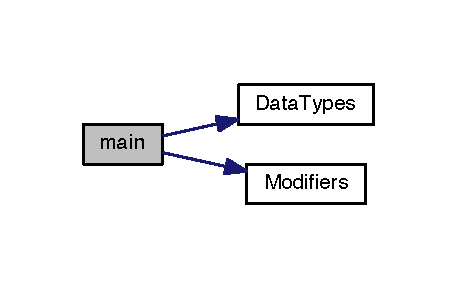
\includegraphics[width=220pt]{_teacher_basics_8c_ae66f6b31b5ad750f1fe042a706a4e3d4_cgraph}
\end{center}
\end{figure}


\hypertarget{_teacher_basics_8c_a6ef0cf8d139194a7cc30e0c64e09b14e}{\index{Teacher\+Basics.\+c@{Teacher\+Basics.\+c}!Modifiers@{Modifiers}}
\index{Modifiers@{Modifiers}!Teacher\+Basics.\+c@{Teacher\+Basics.\+c}}
\subsubsection[{Modifiers}]{\setlength{\rightskip}{0pt plus 5cm}void Modifiers (
\begin{DoxyParamCaption}
{}
\end{DoxyParamCaption}
)}}\label{_teacher_basics_8c_a6ef0cf8d139194a7cc30e0c64e09b14e}


<<<<<<< HEAD
Definition at line 108 of file Teacher\+Basics.\+c.
=======
Definition at line 90 of file Teacher\+Basics.\+c.
>>>>>>> master



Referenced by main().


\begin{DoxyCode}
<<<<<<< HEAD
109 \{
110   \textcolor{comment}{//local variable, string}
111   \textcolor{keywordtype}{char} ch[10];                                                          
112   printf(\textcolor{stringliteral}{"\(\backslash\)n There are five basic modifiers: signed, unsigned, short,"}
113   \textcolor{stringliteral}{" long and const-constant. \(\backslash\)n"});
114   \textcolor{keywordtype}{int} i;
115   \textcolor{keywordflow}{do}
116   \{
117     printf(\textcolor{stringliteral}{"Which modifier do you want to learn about? \(\backslash\)n"});
118     scanf(\textcolor{stringliteral}{" %s"}, ch);
119     i=0;
120     
121     \textcolor{comment}{/*}
122 \textcolor{comment}{    * Conditions for user's choice of subject. }
123 \textcolor{comment}{    * Following can be interpreted as a database of req. info. on subject}
124 \textcolor{comment}{    */}
125     \textcolor{keywordflow}{if}(strcmp(ch,\textcolor{stringliteral}{"signed"})==0) 
126     printf(\textcolor{stringliteral}{"All data types are “signed” by default. Signed Data Modifier"}
127     \textcolor{stringliteral}{" implies that the data type variable can store positive values as well"}
128     \textcolor{stringliteral}{" as negative values. \(\backslash\)nFor example: signed int temperature; \(\backslash\)n"}); 
129     \textcolor{keywordflow}{else} \textcolor{keywordflow}{if}(strcmp(ch,\textcolor{stringliteral}{"unsigned"})==0) 
130     printf(\textcolor{stringliteral}{"If we need to change the data type so that it can only store"}
131     \textcolor{stringliteral}{" only store positive values, “unsigned” data modifier is used."}
132     \textcolor{stringliteral}{"\(\backslash\)nFor example: unsigned int salary; \(\backslash\)n"}); 
133     \textcolor{keywordflow}{else} \textcolor{keywordflow}{if}(strcmp(ch,\textcolor{stringliteral}{"short"})==0) 
134     printf(\textcolor{stringliteral}{"A “short” type modifier does"}
135     \textcolor{stringliteral}{" just the opposite of “long”. If one is not expecting to see high range"}
136     \textcolor{stringliteral}{" values in a program and the values are both positive & negative."}
137     \textcolor{stringliteral}{"\(\backslash\)nFor example: short int age; \(\backslash\)n"}); 
138     \textcolor{keywordflow}{else} \textcolor{keywordflow}{if}(strcmp(ch,\textcolor{stringliteral}{"long"})==0) 
139     printf(\textcolor{stringliteral}{"Sometimes while coding a program,"}
140     \textcolor{stringliteral}{" we need to increase the Storage Capacity of a variable so that it can store"}
141     \textcolor{stringliteral}{" values higher than its maximum limit which is there as default. In such"}
142     \textcolor{stringliteral}{" situations or programs, we need to make use of the “long” data type qualifier."}
143     \textcolor{stringliteral}{" “long” type modifier doubles the “length” of the data type when used along with it."}
144     \textcolor{stringliteral}{"\(\backslash\)nFor example: long int turnover; \(\backslash\)n"}); 
145     \textcolor{keywordflow}{else} \textcolor{keywordflow}{if}(strcmp(ch,\textcolor{stringliteral}{"const"})==0) 
146     printf(\textcolor{stringliteral}{"const sets the value of variable as"}
147     \textcolor{stringliteral}{" constants. If the program tries to change the value of a constant variable,"}
148     \textcolor{stringliteral}{" it displays an error. \(\backslash\)nFor example: const int MAX=2;"}
149     \textcolor{stringliteral}{" (Has been declared in the beginning.) \(\backslash\)n"}); 
150     \textcolor{keywordflow}{else} 
151     \{ 
152       \textcolor{comment}{//Repeating the input if an error }
153       printf(\textcolor{stringliteral}{"Input either 'signed', 'unsigned', 'short', 'const' or 'long'. \(\backslash\)n"}); i=1;
154     \}                   
155   \}\textcolor{keywordflow}{while}(i==1);
156   
157 \}\end{DoxyCode}
=======
91 \{
92   \textcolor{comment}{//local variable, string}
93   \textcolor{keywordtype}{char} ch[10];                                                          
94   printf(\textcolor{stringliteral}{"\(\backslash\)n There are five basic modifiers: signed, unsigned, short,"}
95   \textcolor{stringliteral}{" long and const-constant. \(\backslash\)n"});
96   \textcolor{keywordtype}{int} i;
97   \textcolor{keywordflow}{do}
98   \{
99     printf(\textcolor{stringliteral}{"Which modifier do you want to learn about? \(\backslash\)n"});
100     scanf(\textcolor{stringliteral}{" %s"}, ch);
101     i=0;
102     
103     \textcolor{comment}{/*}
104 \textcolor{comment}{    * Conditions for user's choice of subject. }
105 \textcolor{comment}{    * Following can be interpreted as a database of req. info. on subject}
106 \textcolor{comment}{    */}
107     \textcolor{keywordflow}{if}(strcmp(ch,\textcolor{stringliteral}{"signed"})==0) 
108     printf(\textcolor{stringliteral}{"All data types are “signed” by default. Signed Data Modifier"}
109     \textcolor{stringliteral}{" implies that the data type variable can store positive values as well"}
110     \textcolor{stringliteral}{" as negative values. \(\backslash\)nFor example: signed int temperature; \(\backslash\)n"}); 
111     \textcolor{keywordflow}{else} \textcolor{keywordflow}{if}(strcmp(ch,\textcolor{stringliteral}{"unsigned"})==0) 
112     printf(\textcolor{stringliteral}{"If we need to change the data type so that it can only store"}
113     \textcolor{stringliteral}{" only store positive values, “unsigned” data modifier is used."}
114     \textcolor{stringliteral}{"\(\backslash\)nFor example: unsigned int salary; \(\backslash\)n"}); 
115     \textcolor{keywordflow}{else} \textcolor{keywordflow}{if}(strcmp(ch,\textcolor{stringliteral}{"short"})==0) 
116     printf(\textcolor{stringliteral}{"A “short” type modifier does"}
117     \textcolor{stringliteral}{" just the opposite of “long”. If one is not expecting to see high range"}
118     \textcolor{stringliteral}{" values in a program and the values are both positive & negative."}
119     \textcolor{stringliteral}{"\(\backslash\)nFor example: short int age; \(\backslash\)n"}); 
120     \textcolor{keywordflow}{else} \textcolor{keywordflow}{if}(strcmp(ch,\textcolor{stringliteral}{"long"})==0) 
121     printf(\textcolor{stringliteral}{"Sometimes while coding a program,"}
122     \textcolor{stringliteral}{" we need to increase the Storage Capacity of a variable so that it can store"}
123     \textcolor{stringliteral}{" values higher than its maximum limit which is there as default. In such"}
124     \textcolor{stringliteral}{" situations or programs, we need to make use of the “long” data type qualifier."}
125     \textcolor{stringliteral}{" “long” type modifier doubles the “length” of the data type when used along with it."}
126     \textcolor{stringliteral}{"\(\backslash\)nFor example: long int turnover; \(\backslash\)n"}); 
127     \textcolor{keywordflow}{else} \textcolor{keywordflow}{if}(strcmp(ch,\textcolor{stringliteral}{"const"})==0) 
128     printf(\textcolor{stringliteral}{"const sets the value of variable as"}
129     \textcolor{stringliteral}{" constants. If the program tries to change the value of a constant variable,"}
130     \textcolor{stringliteral}{" it displays an error. \(\backslash\)nFor example: const int MAX=2;"}
131     \textcolor{stringliteral}{" (Has been declared in the beginning.) \(\backslash\)n"}); 
132     \textcolor{keywordflow}{else} 
133     \{ 
134       \textcolor{comment}{//Repeating the input if an error }
135       printf(\textcolor{stringliteral}{"Input either 'signed', 'unsigned', 'short', 'const' or 'long'. \(\backslash\)n"}); i=1;
136     \}                   
137   \}\textcolor{keywordflow}{while}(i==1);
138   
139 \}\end{DoxyCode}
>>>>>>> master


Here is the caller graph for this function\+:\nopagebreak
\begin{figure}[H]
\begin{center}
\leavevmode
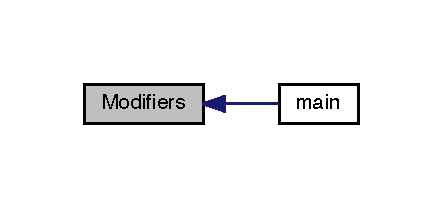
\includegraphics[width=212pt]{_teacher_basics_8c_a6ef0cf8d139194a7cc30e0c64e09b14e_icgraph}
\end{center}
\end{figure}




\subsection{Variable Documentation}
\hypertarget{_teacher_basics_8c_af7dbda7167e22cb3417c16f78061ad80}{\index{Teacher\+Basics.\+c@{Teacher\+Basics.\+c}!M\+A\+X@{M\+A\+X}}
\index{M\+A\+X@{M\+A\+X}!Teacher\+Basics.\+c@{Teacher\+Basics.\+c}}
\subsubsection[{M\+A\+X}]{\setlength{\rightskip}{0pt plus 5cm}const int M\+A\+X =2}}\label{_teacher_basics_8c_af7dbda7167e22cb3417c16f78061ad80}


Definition at line 5 of file Teacher\+Basics.\+c.


%--- End generated contents ---

% Index
\newpage
\phantomsection
\addcontentsline{toc}{chapter}{Index}
\printindex

\end{document}
